\chapter{Realtà Virtuale}
\label{VR}

%Nella seconda sezione si riporta lo stato dell'arte del settore, un inquadramento dell'area di ricerca orientato a portare il lettore all'interno della problematica affrontata. Bisogna dimostrare di conoscere le cose fatte fino ad ora in questo campo e il perchè si sia reso necessario lo svolgimento di questo lavoro.
 \begin{figure}[htb]
    \centering
    %\vspace{-0.7cm}
    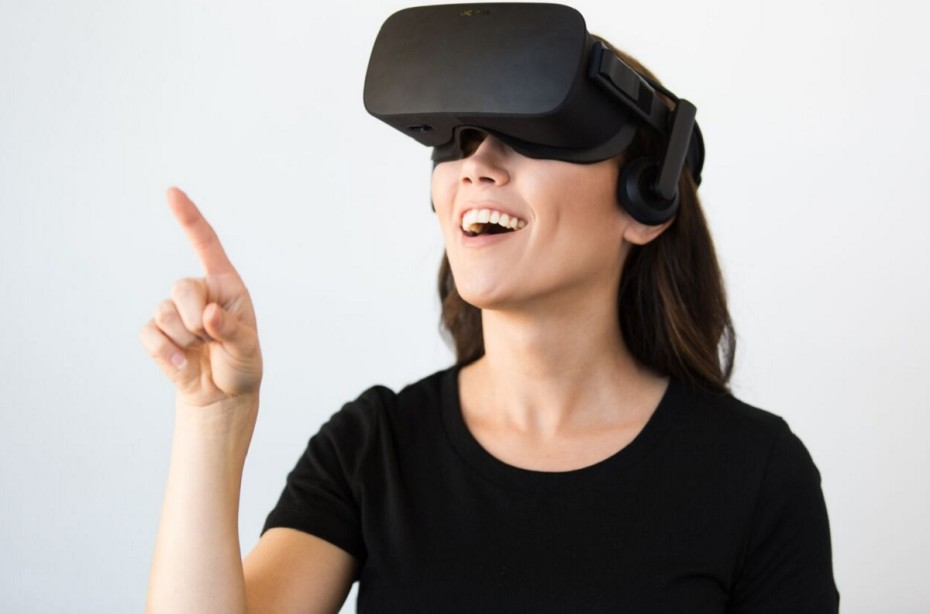
\includegraphics[width=\textwidth]{VR}
    %\vspace{-0.3cm}
\end{figure}
\noindent Ultimamente si parla sempre più spesso di \textit{Realtà Virtuale} ma cos'è, come si crea e a cosa serve?
Il termine \textit{Realtà Virtuale} fu coniato nel 1989 da Jaron Lanier, una delle prime persone che iniziò a lavorarci. Con il termine Realtà virtuale (Virtual Reality) si indica una Realtà simulata che si realizza attraverso la ricostruzione di ambienti o oggetti in modo da dare al soggetto una percezione il più possibile realistica della loro esistenza. A questa definizione tecnica si può a affiancare una più generale, che vede la Realtà virtuale come una Realtà parallela. È possibile distinguere due tipi di Realtà virtuale: una immersiva e una non immersiva. Si definisce immersiva la Realtà virtuale che è in grado di assorbire l'utente, realizzando una vera e propria immersione dei sensi nell'ambiente tridimensionale generato dal computer. Ciò è possibile attraverso l'utilizzo di dispositivi particolari: un visore, che permette la visualizzazione delle immagini tridimensionali e l'isolamento dall'ambiente esterno, ed un tracker, per il rilevamento di posizione e movimento dell'utente. Oltre a questi ne esistono molti altri, di cui alcuni ancora in fase di studio e perfezionamento. La Realtà virtuale non immersiva, invece, è caratterizzata dall'utilizzo di un monitor per la visualizzazione delle immagini tridimensionali e non si serve dell'ausilio di un tracker determinando nell'utente la sensazione di vedere il mondo tridimensionale, creato dal computer, come attraverso "una finestra" e in maniera quindi non partecipativa.
\section{Come si crea la Realtà Virtuale}
La Realtà Virtuale è possibile grazie a strumenti, programmi e linguaggi di programmazione appositi. Nella tesi proposta, si è scelto di utilizzare una Realtà Virtuale di tipo immersivo. Questa tipologia richiede una strumentazione più complessa e performante rispetto alla tipologia non immersiva. Gli strumenti che richiede, sono i seguenti:
\begin{itemize}
  \item \textbf{Computer}: tutte le periferiche utilizzate fanno capo a un hardware, se non integrato, che funge da fulcro per l’elaborazione e lo smistamento dei dati. Questo fulcro è spesso rappresentato da un computer dalle prestazioni elevate, in termini di CPU e GPU. La sua funzione, oltre a mantenere uno stato aggiornato, è quella di ricevere dati da sensori esterni, utili per recepire le azioni dell’utilizzatore, e inviare informazioni di feedback delle azioni elaborate. Ad esempio l’aggiornamento delle immagini visualizzate e l’attivazione di attuatori per altri tipi di sensazioni (ad esempi tattili).
	\item\textbf{Visore}: costituito da due pannelli LCD impostati per la vista bioculare, questo isola dal mondo esterno e costituisce una specie di casco. Questa impostazione dà la sensazione di tridimensionalità. Il visore può essere dotato di sensori in grado di rilevare i movimenti dell’utente come la rotazione del capo per inquadrare un’altra area del mondo virtuale. In alternativa, esistono visori economici che non sono altro che contenitori, muniti di lenti, che permettono di inserire lo smartphone e utilizzarlo come schermo LCD e come fulcro di tutte le funzioni hardware e software.
  \item \textbf{Auricolari}: solitamente integrati nei visori, permettono di udire i suoni emessi dal mondo virtuale. Il software deve variare i suoni emessi in base alla posizione dell'utilizzatore.
  \item \textbf{Sensori}: per il riconoscimento dei movimenti e delle azioni dell'utilizzatore. I sensori presenti nel visore danno informazioni sulla posizione, sul movimento della testa e del corpo. I sensori sono di vario tipo e sono in continuo sviluppo. I più conosciuti sono: guanti, in sostituzione dei canonici gestori di input (joystick, mouse, tastiere, ecc.); tute, in grado di trasferire le posture e i movimenti dell’utente nella rappresentazione e Virtuix Omni, una piattaforma che permette di muoversi camminando nell’ambiente virtuale.
\end{itemize}






















%